\documentclass{article}
\usepackage{amsmath,amssymb,mathrsfs,amsthm,graphicx}
%\usepackage{tikz-cd}
\usepackage{hyperref}
\newcommand{\inner}[2]{\left\langle #1, #2 \right\rangle}
\newcommand{\tr}{\ensuremath\mathrm{tr}\,} 
\newcommand{\Span}{\ensuremath\mathrm{span}} 
\def\Re{\ensuremath{\mathrm{Re}}\,}
\def\Im{\ensuremath{\mathrm{Im}}\,}
\newcommand{\id}{\ensuremath\mathrm{id}} 
\newcommand{\var}{\ensuremath\mathrm{var}} 
\newcommand{\Lip}{\ensuremath\mathrm{Lip}} 
\newcommand{\GL}{\ensuremath\mathrm{GL}} 
\newcommand{\diam}{\ensuremath\mathrm{diam}} 
\newcommand{\sgn}{\ensuremath\mathrm{sgn}\,} 
\newcommand{\lcm}{\ensuremath\mathrm{lcm}} 
\newcommand{\supp}{\ensuremath\mathrm{supp}\,}
\newcommand{\dom}{\ensuremath\mathrm{dom}\,}
\newcommand{\upto}{\nearrow}
\newcommand{\downto}{\searrow}
\newcommand{\norm}[1]{\left\Vert #1 \right\Vert}
\newtheorem{theorem}{Theorem}
\newtheorem{lemma}[theorem]{Lemma}
\newtheorem{proposition}[theorem]{Proposition}
\newtheorem{corollary}[theorem]{Corollary}
\theoremstyle{definition}
\newtheorem{definition}[theorem]{Definition}
\newtheorem{example}[theorem]{Example}
\begin{document}
\title{The $C^\infty$ Urysohn lemma}
\author{Jordan Bell\\ \texttt{jordan.bell@gmail.com}\\Department of Mathematics, University of Toronto}
\date{\today}

\maketitle

Define $\eta:\mathbb{R} \to \mathbb{R}$ by
\[
\eta(t) = e^{-1/t} 1_{(0,\infty)}(t).
\]
It is a fact that $\eta$ is $C^\infty$. This is proved by showing that for each $k \geq 1$ there is a polynomial $P_k$ of degree $2k$ such that $\eta^{(k)}(t)=P_k(t^{-1}) e^{-1/t}$ for
$t>0$, and that $\eta^{(k)}(0)=0$, which together imply that $\eta \in C^k$.


Define $\psi:\mathbb{R}^d \to \mathbb{R}$ by
\[
\psi(x) = \eta(1-|x|^2) = \begin{cases}
e^{\frac{1}{|x|^2-1}}&|x|<1\\
0&|x| \geq 1.
\end{cases}
\]
Because $x \mapsto 1-|x|^2$ is $C^\infty:\mathbb{R}^d \to \mathbb{R}$,  the chain rule tells us that
$\psi$ is $C^\infty$. 

For a function $\phi$ on $\mathbb{R}^d$ and for $t>0$, we define
\[
\phi_t(x) = t^{-d} \phi(t^{-1}x).
\]

We now construct bump functions.\footnote{The following construction of a bump function 
follows  Gerald B. Folland, {\em Real Analysis: Modern Techniques
and Their Applications}, second ed., p.~245, Lemma 8.18.}


\begin{theorem}[$C^\infty$ Urysohn lemma]
If $K$ is a compact subset of $\mathbb{R}^d$ and $U$ is an open set containing $K$,
then there exists $\phi \in C^\infty(\mathbb{R}^d)$ with $0 \leq \phi \leq 1$, $\phi=1$ on $K$,
and $\supp \phi \subset U$. Moreover, if $K$ is invariant under $SO(d)$ then the function $\phi$ constructed here
is radial.
\end{theorem}
\begin{proof}
Let
\[
\delta = d(K,U^c),
\]
which is positive 
because $K$ is compact and $U^c$ is closed.
Let
\[
V=\left\{x \in \mathbb{R}^d: d(x,K)<\frac{\delta}{3}\right\} = K+B_{\delta/3},
\]
and define $f$ on $\mathbb{R}^d$ by
\[
f = \left(\int_{\mathbb{R}^d} \psi(x) dx \right)^{-1} \psi_{\delta/3},
\]
whose support is
\[
\supp f = \supp \psi_{\delta/3} = \overline{B_{\delta/3}}.
\]
Finally define $\phi$ on $\mathbb{R}^d$ by
\[
\phi = 1_V * f.
\]
Because $V$ is bounded and $f$ is $C^\infty$, the function $\phi$ is $C^\infty$. 
The support of $\phi$ is
\[
\supp \phi = \supp(1_V*f) \subset \overline{\supp 1_V + \supp f}
=\overline{V+ \overline{B_{\delta/3}}}
=K+\overline{B_{2\delta/3}} \subset U.
\]
Because $1_V$ and $f$ are nonnegative, so is their convolution $\phi$. 
For any $x$,
\[
\phi(x) = \int_{\mathbb{R}^d} 1_V(x-y) f(y) dy
\leq \int_{\mathbb{R}^d} f(y) dy = 1,
\]
so $0 \leq \phi \leq 1$. 
For $x \in K$, if $y \in V^c$ then 
$|x-y| \geq \delta/3$.
But $f(u)=0$ for $|u| \geq \delta/3$, so in this case $f(x-y)=0$. 
This implies that for $x \in K$ the functions
$y \mapsto 1_V(y) f(x-y)$ and $y \mapsto f(x-y)$ are equal, hence
\[
\phi(x) = \int_{\mathbb{R}^d} 1_V(y) f(x-y) dy
=\int_{\mathbb{R}^d} f(x-y) dy
=\int_{\mathbb{R}^d} f(y) dy = 1.
\]
This shows that $\phi=1$ on $K$,  verifying all the assertions made about $\phi$.

The function $\psi$ is radial and so $f$ is too.
If $V$ is invariant under $SO(d)$, then the indicator function $1_V$ is radial. Thus, if $K$ is invariant under $SO(d)$ 
then $1_V$ is radial, and 
the convolution of two radial functions is also radial, which means that $\phi$ is  radial in this case.
\end{proof}


For example, take $d=1$, take
 $K$ to be the closed ball of radius $1$, and take  $U$ to be the open ball of radius $2$.
 Then $\delta=d(K,U^c) = 1$ and $V=B_{4/3}$. 
 In Figure \ref{urysohn} we plot the bump function $\phi$ constructed in the above theorem.
 
 
\begin{figure}
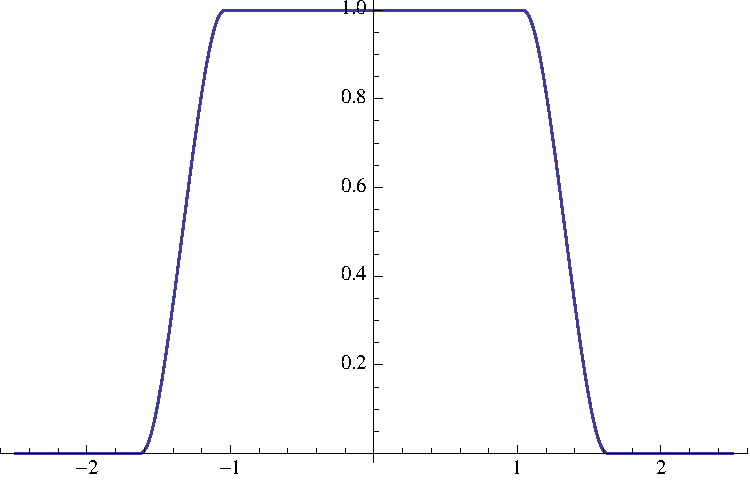
\includegraphics[scale=0.80]{phi}
\caption{The bump function $\phi$, for $d=1$, $K=[-1,1]$, $U=(-2,2)$; $\delta=1$ and $V=(-4/3,4/3)$}
\label{urysohn}
\end{figure}



\end{document}